\documentclass[11pt]{charter}

% El títulos de la memoria, se usa en la carátula y se puede usar el cualquier lugar del documento con el comando \ttitle
\titulo{Sistema de monitoreo de temperaturas en tiempo real para refrigeradores críticos de salud} 

% Nombre del posgrado, se usa en la carátula y se puede usar el cualquier lugar del documento con el comando \degreename
%\posgrado{Carrera de Especialización en Sistemas Embebidos} 
\posgrado{Carrera de Especialización en Internet de las Cosas} 
%\posgrado{Carrera de Especialización en Intelegencia Artificial}
%\posgrado{Maestría en Sistemas Embebidos} 
%\posgrado{Maestría en Internet de las cosas}

% Tu nombre, se puede usar el cualquier lugar del documento con el comando \authorname
\autor{Marcelo Castello} 

% El nombre del director y co-director, se puede usar el cualquier lugar del documento con el comando \supname y \cosupname y \pertesupname y \pertecosupname
\director{Juan José Salerno}
\pertenenciaDirector{Dirección de Bioingeniería} 
% FIXME:NO IMPLEMENTADO EL CODIRECTOR ni su pertenencia
\codirector{} % si queda vacio no se deberíá incluir 
\pertenenciaCoDirector{}

% Nombre del cliente, quien va a aprobar los resultados del proyecto, se puede usar con el comando \clientename y \empclientename
\cliente{Edgardo Marino}
\empresaCliente{Municipalidad de Rosario}

% Nombre y pertenencia de los jurados, se pueden usar el cualquier lugar del documento con el comando \jurunoname, \jurdosname y \jurtresname y \perteunoname, \pertedosname y \pertetresname.
\juradoUno{Nombre y Apellido (1)}
\pertenenciaJurUno{pertenencia (1)} 
\juradoDos{Nombre y Apellido (2)}
\pertenenciaJurDos{pertenencia (2)}
\juradoTres{Nombre y Apellido (3)}
\pertenenciaJurTres{pertenencia (3)}
 
\fechaINICIO{25 de agosto de 2020}		%Fecha de inicio de la cursada de GdP \fechaInicioName
\fechaFINALPlanificacion{6 de octubre de 2020} 	%Fecha de final de cursada de GdP
\fechaFINALTrabajo{25 de agosto de 2021}		%Fecha de defensa pública del trabajo final


\begin{document}

\maketitle
\thispagestyle{empty}
\pagebreak


\thispagestyle{empty}
{\setlength{\parskip}{0pt}
\tableofcontents{}
}
\pagebreak


\section{Registros de cambios}
\label{sec:registro}


\begin{table}[ht]
\label{tab:registro}
\centering
\begin{tabularx}{\linewidth}{@{}|c|X|c|@{}}
\hline
\rowcolor[HTML]{C0C0C0} 
Revisión & \multicolumn{1}{c|}{\cellcolor[HTML]{C0C0C0}Detalles de los cambios realizados} & Fecha      \\ \hline
1.0      & Creación del documento \newline Versión inicial: propósito, alcance, supuestos, requerimientos, entregables y desglose del trabajo.
                                         & 26/08/2020 \\ \hline
%1.1      &                                                                 & dd/mm/aaaa \\ \hline
%1.2      & Otro ejemplo \newline
%		   Con texto partido \newline
%		   En varias líneas \newline
%		   A propósito                                                     & dd/mm/aaaa \\ \hline
\end{tabularx}
\end{table}

\pagebreak



\section{Acta de constitución del proyecto}
\label{sec:acta}

\begin{flushright}
Buenos Aires, \fechaInicioName
\end{flushright}

\vspace{2cm}

Por medio de la presente se acuerda con el Ing. \authorname\hspace{1px} que su Trabajo Final de la \degreename\hspace{1px} se titulará ``\ttitle'', consistirá esencialmente en el prototipo preliminar de un sistema para la medición, visualización y emisión de alertas de temperatura para heladeras y freezers en bancos de sangre y vacunatorios de efectores de salud de la Municipalidad de Rosario, y tendrá un presupuesto preliminar estimado de 638 hs de trabajo y \textcolor{red}{\$XXX}, con fecha de inicio \fechaInicioName\hspace{1px} y fecha de presentación pública \fechaFinalName.

Se adjunta a esta acta la planificación inicial.

\vfill

% Esta parte se construye sola con la información que hayan cargado en el preámbulo del documento y no debe modificarla
\begin{table}[ht]
\centering
\begin{tabular}{ccc}
\begin{tabular}[c]{@{}c@{}}Ariel Lutenberg \\ Director posgrado FIUBA\end{tabular} & \hspace{2cm} & \begin{tabular}[c]{@{}c@{}}\clientename \\ \empclientename \end{tabular} \vspace{2.5cm} \\ 
\multicolumn{3}{c}{\begin{tabular}[c]{@{}c@{}} \supname \\ Director del Trabajo Final\end{tabular}} \vspace{2.5cm} \\
%\begin{tabular}[c]{@{}c@{}}\jurunoname \\ Jurado del Trabajo Final\end{tabular}     &  & \begin{tabular}[c]{@{}c@{}}\jurdosname\\ Jurado del Trabajo Final\end{tabular}  \vspace{2.5cm}  \\
%\multicolumn{3}{c}{\begin{tabular}[c]{@{}c@{}} \jurtresname\\ Jurado del Trabajo Final\end{tabular}} \vspace{.5cm}                                                                     
\end{tabular}
\end{table}




\section{Descripción técnica-conceptual del proyecto a realizar}
\label{sec:descripcion}

\begin{consigna}{black}
%El objetivo es que el lector en una o dos páginas entienda de qué se trata el proyecto y cuáles son sus desafíos, su motivación y su importancia.
%Se debe destacar claramente cuál es el valor que agrega el proyecto a realizar. ``El presente proyecto se destaca especialmente por incorporar tal cosa... Esto lo diferencia de otros sistemas similares en que ...''
El buen funcionamiento de los sistemas de refrigeración es afectado a menudo por cortes de energía, mermas en el rendimiento del equipo compresor, o pérdidas en el sello ya sea por desgaste de burletes o puertas no bien cerradas.
En el área de salud esto resulta crítico. Productos medicinales como hemoproductos o vacunas, pueden perder la eficacia médica. Esto no sólo se traduce en pérdidas económicas, sino también implica que los tratamientos sobre las personas pueden no ser efectivos o que no puedan ser accedidos por la pérdida del material, con el consecuente impacto social y mediático que esto representa en una empresa pública. 

%Los cortes de energía que se producen a menudo en la red eléctrica afectan de manera directa el buen funcionamiento de los sistemas de refrigeración, sean de productos medicinales como de hemoproductos, pudiendo en algunos casos perder la cadena de frío con la consiguiente pérdida del material almacenado. Esto no sólo se traduce en pérdidas económicas, sino también implica que personas no puedan acceder a los tratamientos o vacunas con el consecuente impacto social y mediático que esto representa en una empresa pública. 
Además la Administración Nacional de Medicamentos Alimentos y Tecnología Médica (ANMAT), a través de la disposición: "Reglamento Técnico Mercosur sobre Buenas Prácticas de Distribución de Productos Farmacéuticos", Resolución Mercosur GMC Nº 49/2002, define un conjunto de prácticas para el transporte y almacenamiento de productos farmacéuticos donde exige trazabilidad, equipamiento para el control y registro continuo de temperaturas con el fin de asegurar las condiciones ambientales de almacenamiento de tales productos. 

La medición a distancia continua y en tiempo real de estas temperaturas sumado a un sistema de alerta, aseguran las condiciones legales, minimizan los riesgos y garantizan la disponibilidad de hemoproductos y vacunas seguros en el momento y el lugar en que se precise. 

Este tabajo se enmarca en dos premisas fundamentales:
\begin{itemize}
\item Las políticas escenciales de la Secretaría de Salud Pública cuya misión es preservar la salud de la población, proponiendo un trabajo integrador para la construcción de opciones y entornos saludables.
\item El contexto sanitario mundial de hoy exige que en un futuro cercano se puedan distribuir adecuadamente y de manera segura especialidades medicinales tales como las vacunas.
\end{itemize}
Los equipos y software de que se dispone en plaza en su mayoría son de origen extranjero, y su utilización -además de onerosa- implica una dependencia con los fabricantes, en términos económicos pero también de criterios (en general se comercializan por módulos, no proveyendo soluciones integrales). En otras palabras, para trabajar con estos recursos se deben seguir criterios técnico-económicos diseñados para otras latitudes y otras condiciones. Se deben realizar adaptaciones y aproximaciones que implican tareas adicionales y que no siempre son del todo efectivas. El personal destinado a estas tareas debe entrenarse utilizando tiempo y esfuerzo, y este entrenamiento debe reforzarse cada vez que el propietario del sistema decide algún cambio o actualización. En el desarrollo de la presente idea, se ha pensado que tal vez este esfuerzo podría ser redirigido a tareas más provechosas.
Se requiere entonces el desarrollo de tecnología propia destinada a este fin, que pueda ser adaptada a las necesidades de los investigadores locales, evitando la dependencia tecnológica en equipos y en software, y reduciendo en todo lo posible las erogaciones durante la investigación por este ítem.

Desde el punto de vista tecnológico el presente proyecto se destaca especialmente por incorporar una solución integral sin gastos de abono y con la característica distintiva que los datos están guardados en los servidores del cliente. Esto lo diferencia de otros sistemas similares en que los datos quedan en poder del fabricante, quien eventualmente, nos ofrece un portal para poder hacer una visualización, además al no ofrecer una solución integral, cada módulo extra incorporado, representa un gasto o abono adicional. 

La solución propuesta se compone de las siguientes partes:
\begin{itemize}
\item Medición de la temperatura
\item Transporte de los datos
\item Lógica de procesamiento y persistencia de datos
\item Visualización y alarmas
\end{itemize}
%Puede ser útil incluir en esta sección la respuesta a alguna de estas preguntas:


%La descripción técnica-conceptual \textbf{debe incluir al menos un diagrama en bloques del sistema }y una frase como la siguiente: ``En la Figura \ref{fig:diagBloques} se presenta el diagrama en bloques del sistema. Se observa que...''. Luego recién más abajo de haber puesto esta frase se pone la figura. La regla es que las figuras nunca pueden ir antes de ser mencionadas en el texto, porque sino el lector no entiende por qué de pronto aparece una figura.
En la figura 1 se observa un diagrama en bloques general del sistema, donde se aprecia que los sensores estarán ubicados en distintos efectores del sistema de salud municipal en las áreas de hemoterapia y vacunación. Además se puede ver el sistema de almacenamiento y visualización implementado con un tablero de control  (dashboard) en un servidor centralizado ubicado en el datacenter de la Secretaría de Salud Pública. Por simplicidad, se han dibujado sólo tres efectores. Es necesario destacar que el sistema de salud pública municipal de la ciudad de Rosario consta de 6 hospitales, un centro de especialidades médicas, un centro regional de sangre una droguería central y 50 centros de atención primaria de la salud.
\vspace{25px}

\begin{figure}[htpb]
\centering 
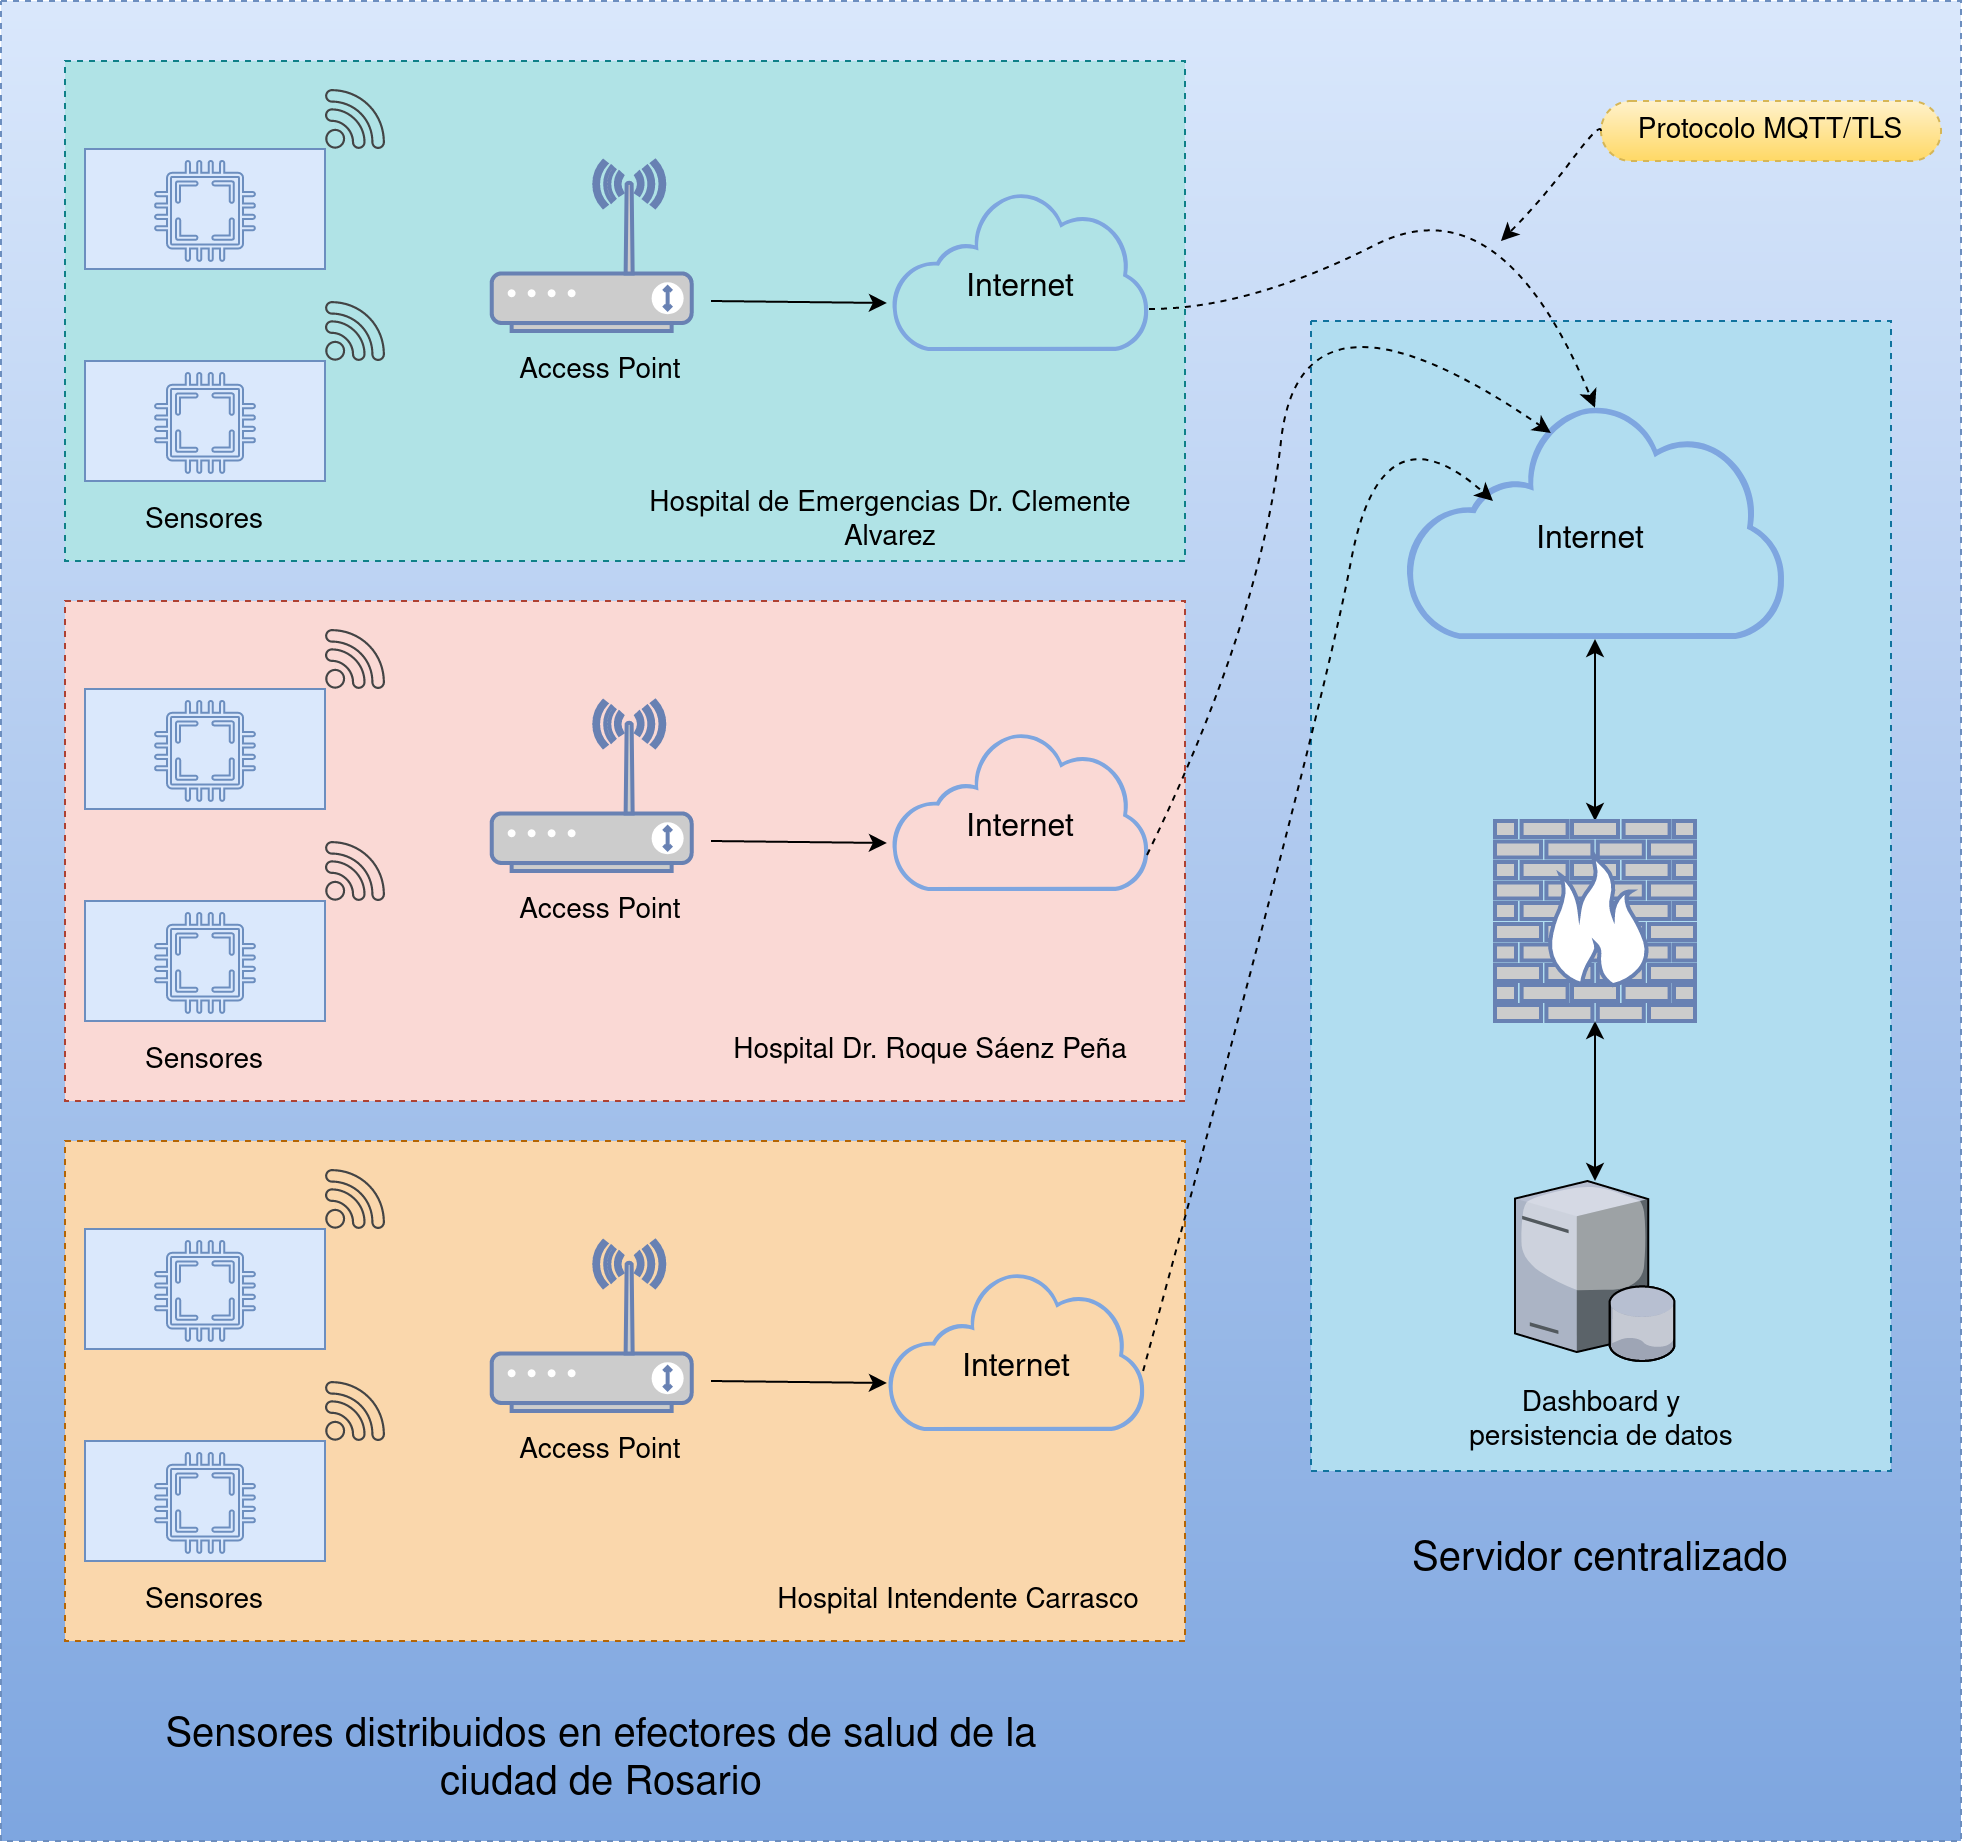
\includegraphics[width=.7\textwidth]{./Figuras/bloquesgral.png}
\caption{Diagrama en bloques del sistema}
\label{fig:diagBloques}
\end{figure}

\vspace{25px}

%El tamaño de la tipografía en la figura debe ser adecuado para que NO pase lo que ocurre acá, donde el lector debe esforzarse para poder leer el texto. Los colores usados en el diagrama deben ser adecuados, tal que ayuden a comprender mejor el diagrama.
\end{consigna}


\section{Identificación y análisis de los interesados}
\label{sec:interesados}

\begin{consigna}{black} 
%Nota: (borrar esto y todas las consignas en color rojo antes de entregar este documento).
 
%Es inusual que una misma persona esté en más de un rol, incluso en proyectos chicos.
 
%Si se considera que una persona cumple dos o más roles, entonces sólo dejarla en el rol más importante. Por ejemplo:

%\begin{itemize}
%\item Si una persona es Cliente pero también colabora u orienta, dejarla solo como Cliente.
%\item Si una persona es el Responsable, no debe ser colocado también como Miembro del equipo.
%\end{itemize}

%Pero en cambio sí es usual que el Cliente y el Auspiciante sean el mismo, por ejemplo.

\begin{table}[ht]
%\caption{Identificación de los interesados}
%\label{tab:interesados}
\begin{tabularx}{\linewidth}{@{}|l|X|X|l|@{}}
\hline
\rowcolor[HTML]{C0C0C0} 
Rol           & Nombre y Apellido & Organización 	& Puesto 	\\ \hline
%Auspiciante   &                   &              	&    -    	\\ \hline
Cliente       & \clientename      &\empclientename	&      Director de Bioingeniería\\ \hline
Impulsor y colaborador      & Roberto Collelo  & Secretaría de Salud Pública	&Sub Director de Bioingeniería\\ \hline
Responsable   & \authorname       & FIUBA        	& Alumno 	\\ \hline
Colaboradores & 
                Silvana Pereyra &Dirección Centros de Salud	 &Jefa Droguería Central\\ \hline
Orientador    & \supname	      & \pertesupname 	& Director	Trabajo final \\ \hline
%Equipo        & miembro1 \newline 
%				miembro2          &       -       	&      -  	\\ \hline
%Opositores    &    -               &      -        	&     -   	\\ \hline
%Usuario final &      -             &      -        	&      -  	\\ \hline
\end{tabularx}
\end{table}


%Sería deseable listar a continuación de la tabla las principales características de cada interesado.
 
%Por ejemplo:
\begin{itemize}
%\item Auspiciante: es riguroso y exigente con la rendición de gastos. Tener mucho cuidado con esto.
%\item Equipo: Juan Perez, suele pedir licencia porque tiene un familiar con una enfermedad. Planificar considerando esto.
\item Colaboradores

Roberto Collelo, resulta de valiosa ayuda en el desarrollo del firmware de los sensores, además de promover el proyecto en las estructuras de mando de la Secretaría de Salud Pública.

Silvana Pereyra, su intervención será desde el lado usuarios, ya que se muestra como una facilitadora para la implementación del sistema.
\end{itemize}

\end{consigna}



\section{1. Propósito del proyecto}
\label{sec:proposito}

\begin{consigna}{black}
El propósito de este proyecto es poner en marcha un sistema de registro y visualización de temperaturas para refrigeradores críticos del área salud, con el objetivo de minimizar los riesgos de pérdida de material, mantener la calidad y eficacia médica de los productos, asegurando las condiciones legales exigidas por la autoridad.
\end{consigna}

\section{2. Alcance del proyecto}
\label{sec:alcance}

\begin{consigna}{black}
El presente proyecto incluye el desarrollo de sus partes fundamentales para que sea capaz de tener una vigilancia de temperatura de al menos 4 heladeras pertenecientes a distintos efectores de salud de la ciudad de Rosario. 
Para ello se desarrollarán y producirán las placas de circuito impreso para los sensores de temperatura, se integrarán en una caja plástica para poder ser colocados en el equipamiento a monitorear.

Se instalará y configurará en un servidor con sistema operativo GNU/Linux con distribución Debian, la dashboard Thingsboard versión Community Edition que es la versión libre de licenciamientos pero que contiene todas las funcionalidades necesarias para este proyecto.

Se configurarán reglas en la dashboard para comparar las temperaturas de los dispositivos con sus rangos para así originar las alarmas y enviar las notificaciones.

Se instalará una base de datos en el servidor central donde se almacenarán las temperaturas, y las configuraciones del sistema.

Se configurarán en la dashboard paneles para que proporcionen información de temperatura y estado para cada dispositivo conectado al sistema.

Las notificaciones de alarmas se harán por medio de la red Telegram, configurando un canal para cada efector/área.


El presente proyecto no incluye la provisión de la infraestructura de transporte de datos, esto es, los equipos para puntos de acceso a internet y las conexiones a internet para cada área donde estarán emplazados los sensores. Tampoco incluirá certificaciones emitidas por las autoridades competentes.
Los sensores desarrollados no son aptos para su instalación en equipos ultrafreezer (-70º).
Los sensores no almacenarán los valores de temperaruras en memorias externas tipo SD ni en la memoria interna del microcontrolador.
Los sensores no usarán baterías para su funcionamiento.

\end{consigna}


\section{3. Supuestos del proyecto}
\label{sec:supuestos}

\begin{consigna}{black}
Para el desarrollo del presente proyecto se supone que:

\begin{itemize}
\item Las áreas donde se colocarán los sensores deberán disponer de una conexión a internet.
\item Para la puesta en producción, se utilizará la infraestructura de servidores de la red informática metropolitana de la ciudad de Rosario
\item Los recursos humanos y el tiempo necesario para el desarollo, serán proporcionados por la Municipalidad de Rosario.
\item El gasto producido por la compra de los elementos necesarios será proporcionado por la Municipalidad de Rosario.
\end{itemize}

\end{consigna}

\section{4. Requerimientos}
\label{sec:requerimientos}

\begin{consigna}{black}
Se presentan a continuación los requerimientos del proyecto, los mismos están presentados en funcionales y no funcionales, donde los ítems de cada requerimiento están priorizados por orden de aparición.

Estos requerimientos se obtuvieron por:
\begin{itemize}
\item Relevamiento de las espectativas de los usuarios.
\item Relevamiento de las condiciones impuestas por el cliente.
\item Estudio de los elementos electrónicos disponibles en el mercado local y extranjero.
\item Ordenanza de contabilidad de la Municipalidad de Rosario.
\end{itemize}

\begin{enumerate}
\item Requerimientos de hardware de los sensores
	\begin{enumerate}
	\item El microcontrolador utilizado deberá estar en fase de producción activa.
	\item El microcontrolador deberá contener capa física WiFi.	
	\item El elemento sensor deberá tener un rango de medición entre -50 y 100 ºC
	\item Deberá incluir en su circuito un filtro activo para la entrada de temperatura.
	\item Deberá incorporar leds de conexión y rango.	
	\end{enumerate}
	
\item Requerimientos del software de los sensores
	\begin{enumerate}
	\item Deberá contener un conjunto de parámetros que identifiquen de forma unívoca el sensor dentro del sistema.	
	\item Los parámetros se deberán almacenar en memoria no volátil.
	\item Deberá gestionar el procesamiento de los valores de temperatura: muestreo cada segundo y promediado cada 600 segundos.	
	\item Se deberá incorporar una página web para configuración de parámetros específicos del sensor.
	\item Deberá incorporar un sistema de actualización remota del firmware.
    \item Deberá ser capaz de conectar distintos modelos de sensores de temperatura.
	\end{enumerate}	
	
\item Requerimientos de seguridad informática
	\begin{enumerate}
	\item La transmisión de los datos se deberá realizar con encriptación, utilizando para ello protocolos de seguridad.
	\item El acceso al sistema de visualización deberá ser con usuario y contraseña.
	\item El acceso a la página web del sensor deberá ser con usuario y contraseña.
	\end{enumerate}	

\item Requerimientos del cliente
	\begin{enumerate}
	\item El sistema de visualización debe incluir roles para distintos usuarios.
		\begin{enumerate}
		\item Rol Administrador: podrá dar alta a usuarios y cambiar sus roles.
	     \item Rol Jefe: podrá cambiar parámetros, visualizar series de tiempo y recibir alertas.
	     \item Rol Operador: Sólo podrá visualizar series de tiempo y recibir alertas.
	     \end{enumerate}
	\item El sistema deberá prever la incorporación de otras variables a monitorear, que serán materia de desarrollos futuros de sensores.
	\item El sistema de visualización deberá mostrar claramente la estructura jerárquica geográfica de la empresa.	
	\item El sistema deberá ser escalable para implementar nuevas áreas a monitorear.
		\end{enumerate}
		
\item Requerimientos del sistema de visualización
    \begin{enumerate}
	\item Deberá mostrar la temperatura.
	\item Deberá mostrar el estado del dispositivo. (online/fuera de rango)
	\item Deberá mostrar la fecha y hora de la última telemetría enviada al servidor.
	\item Deberá mostrar la configuración de los parámetros de alertas (rangos de temperatura).
	\item Deberá mostrar una vista rápida de los sensores fuera de rango mediante plano en pantalla del área.
	\item Deberá mostrar una tabla con el histórico de alarmas por cada sensor.
    \item Deberá mostrar mediante gráficas la evolución de las temperaturas en el dominio del tiempo con entorno configurable.
    \item Deberá mostrar el lugar de emplazamiento del dispositivo.
	\end{enumerate}	
    

\item Requerimientos de las alarmas
	\begin{enumerate}
	\item Deberá enviar las alarmas discriminadas por efector/área.
	\item Deberá enviar notificaciones ante desplazamientos de la temperatura por encima del rango.
	\item Deberá enviar notificaciones ante desplazamientos de la temperatura por debajo del rango.
	\item Deberá enviar notificaciones ante desconexiones del dispositivo sensor.
	\item Deberá enviar notificaciones ante recupero de la conexión del dispositivo sensor.
	 \end{enumerate}	 

\item Requerimientos de compras
	\begin{enumerate}
	\item Se deberá utilizar la gestión de compras directas para elementos con presupuesto menor a {\$10.000}.
	\item Se deberán realizar las gestiones correspondiente para realizar compras en el exterior.
	\end{enumerate}
	
%\item Requierimientos de normativas
%	\begin{enumerate}
%	\item 
%	\item 
%	\end{enumerate}
		
\end{enumerate}


\end{consigna}

\section{Historias de usuarios (\textit{Product backlog})}
\label{sec:backlog}

\begin{consigna}{black}
%Descripción: En esta sección se deben incluir las historias de usuarios y su ponderación (\textit{history points}). Recordar que las historias de usuarios son descripciones cortas y simples de una característica contada desde la perspectiva de la persona que desea la nueva capacidad, generalmente un usuario o cliente del sistema. La ponderación es un número entero que representa el tamaño de la historia comparada con otras historias de similar tipo.
Se muestran a continuación, las historias de usuarios recopiladas. Al principio se presentan dos épicas y sus correspondientes desgloses emanadas de las máximas autoridades de la empresa.
La ponderación de estas historias se realizó teniendo en cuenta la complejidad y el tiempo necesario en resolverlas (criterios complejidad-volumen). Se elijió para la ello una escala basada en la serie de Fibonacci desde el 0 al 13, donde el 0 representa poco esfuerzo y el 13 alto esfuerzo para lograr el objetivo. 

La siguiente tabla muestra la clasificación de las funcionalidades observadas y su ponderación.


\begin{table}[ht]
%caption{Tabla de ponderación}
\begin{tabularx}{\linewidth}{@{}|l|X|X|l|@{}}
\hline
\rowcolor[HTML]{C0C0C0} 
Funcionalidad solicitada           & Ponderación 	\\ \hline

Visualización de temperatura & 0\\ \hline
Gráficas en tiempo real & 1\\ \hline
Gráficas históricas, alarmas, estados & 3\\ \hline
Mapas, seguridad & 5\\ \hline
No previsto en este proyecto & 13\\ \hline

\end{tabularx}
\end{table}
Luego, se les asignó una prioridad de resolución, (ver tabla) teniendo como premisa que el sistema funcione de forma ininterrumpida. Si el sistema funciona como es debido, se podrán cumplir con las funcionalidades primarias que son la de vigilar, notificar, dar seguridad y visualizar, luego vendrán las otras funcionalidades: emisión de alertas, visualización, etc.

\begin{table}[ht]
%caption{Tabla de prioridades}
%\label{tab:interesados} 
\begin{tabularx}{\linewidth}{@{}|l|X|X|l|@{}}
\hline
\rowcolor[HTML]{C0C0C0}
Funciones           & Prioridad 	\\ \hline
Inherentes a la robustez del sistema & 1 \\ \hline
Inherentes a las notificaciones & 2 \\ \hline
Inherentes a la seguridad & 3 \\ \hline
Inherentes a la visualización de datos &4 \\ \hline

\end{tabularx}
\end{table}




\begin{itemize}
\item EPICA: Como Secretario de Salud Pública Municipal, necesito estar seguro de la buena conservación de las vacunas, para poder informar al estado provincial y nacional la disponibilidad de las mismas.

Desglose
	\begin{itemize}
	\item 
    Como secretario de Salud Pública Municipal deseo poder visualizar en cualquier momento la temperatura de cualquier heladera con el objetivo de asegurarse de que no se deterioren. 
    
Ponderación: 0 Prioridad:
	\end{itemize}
	
	\begin{itemize}
	\item 
	Como secretario de Salud Pública Municipal deseo poder recibir una alarma si alguna de las heladeras superan la temperatura de 4 grados centígrados con el objetivo de poder actuar rápidamente y no se deterioren las vacunas. 
	
Ponderación: 3 Prioridad:
	\end{itemize}

	\begin{itemize}
	\item 
	Como secretario de Salud Pública Municipal deseo poder visualizar en cualquier momento cuántas vacunas hay por heladera con el fin de saber si se pueden reubicar vacunas ante una eventual falla de alguna heladera. 

Ponderación: 13 Prioridad:
	\end{itemize}
\end{itemize}

\begin{itemize}
\item EPICA: Como Director de Infraestructura Hospitalaria, deseo conocer si algún efector de la red presenta problemas en los refrigeradores críticos y así direccionar las acciones necesarias para su correción. 

Desglose

	\begin{itemize}
	\item Como Director de Infraestructura Hospitalaria, necesito visualizar mendiante un mapa interactivo el estado de todos los refrigeradores para poder diagramar las acciones de corrección necesarias.  

Ponderación: 5 Prioridad:
	\end{itemize}

	\begin{itemize}
	\item Como Director de Infraestructura Hospitalaria, necesito recibir notificaciones de las anomalías de los equipos de refrigeración para poder indagar a los responsables de la situación.  

Ponderación: 3 Prioridad:
	\end{itemize}

\end{itemize}


\begin{itemize}
\item EPICA: Como Director de Infraestructura Hospitalaria, deseo que a este sistema se le puedan adicionar otras variables físicas para tener un panel de control completo de todo el equipamiento a mi cargo. 

Desglose

	\begin{itemize}
	\item Como Director de Infraestructura Hospitalaria, deseo conoder el nivel de los tanques de agua de todos los efectores de la Municipalidad, para  
	
Ponderación: 13 Prioridad:
	\end{itemize}

	\begin{itemize}
	\item Como Director de Infraestructura Hospitalaria, deseo conoder el estado de los filtros HEPA de los equipos de aire acondicionado de todos los efectores de la Municipalidad, para 
	
Ponderación: 13 Prioridad:
	\end{itemize}

\end{itemize}

\begin{itemize}
\item Como responsable de mantenimiento necesito conocer la evolución de las temperaturas de los refirgeradores en los últimos 6 meses, para estimar las intervenciones preventivas en tales equipos. 

Ponderación: 3 Prioridad:
\end{itemize}


\begin{itemize}
\item Como operario de mantenimiento necesito que el sistema me envíe inmediatamente un alerta a mi teléfono si hay algún apartamiento de temperaturas, para solucionar rápidamente el desperfecto. 

Ponderación: 3 Prioridad:
\end{itemize}


\begin{itemize}
\item Como encargado de mantenimiento electrónico, necesito saber cuándo un sensor deja de funcionar para inmediatamente proceder a su reparación. 

Ponderación: 3 Prioridad:
\end{itemize}

\begin{itemize}
\item Como encargado de mantenimiento electrónico, necesito poder visualizar el último dato de temperatura enviado al servidor para comprobar la completitud de los datos almacenados

Ponderación: 3 Prioridad:
\end{itemize}


\begin{itemize}
\item Como jefe de seguridad informática, necesito que la comunicación de los sensores se haga con mecanismos de encriptación, para proteger los datos de posibles cambios por intromisiones no desadas. 

Ponderación: 5 Prioridad:
\end{itemize}


\begin{itemize}
\item Como Director de farmacia desearía que el acceso al sistema de visualización sea con usuario y contraseña para poder definir roles de usuarios. 

Ponderación: 5 Prioridad:
\end{itemize}


\begin{itemize}
\item Como director de Bioingeniería, debería tener acceso a los datos históricos de temperatura para evaluar el funcionamiento a largo plazo de los equipos de refrigeración. 

Ponderación:3 Prioridad:
\end{itemize}

\begin{itemize}
\item Como director de Bioingeniería, desearía poder visualizar una tabla con los históricos de alarmas para evaluar la cantidad de fallos del equipo de refrigeración. 

Ponderación: 3 Prioridad:
\end{itemize}


\begin{itemize}
\item Como jefa de droguería, necesito tener en pantalla el histórico de temperaturas de la última semana para visualizar si los productos perdieron la cadena de frío. 

Ponderación: 1 Prioridad:
\end{itemize}

\begin{itemize}
\item Como jefa de droguería, necesito tener acceso a cambiar los rangos de temperatura para poder almacenar diferentes productos en diferentes refrigeradores según las necesidades. 

Ponderación: 3 Prioridad:
\end{itemize}

\begin{itemize}
\item Como técnico hemoterapista de guardia, necesito obtener el reporte de las últimas 24 hs de temperaturas para entregar mi guardia con los productos asegurados en su cadena de frio. 

Ponderación:1 Prioridad:
\end{itemize}

\begin{itemize}
\item Como operario de droguería, necesito que el sistema registre las temperaturas cada 10 minutos para evitar los olvidos y las impresiciones del registro manual. 

Ponderación: 0 Prioridad:
\end{itemize}

\end{consigna}

\section{5. Entregables principales del proyecto}
\label{sec:entregables}

\begin{consigna}{black}
\begin{itemize}
\item Manual de uso
\item Diagrama esquemático
\item Código fuente del firmware de los sensores.
\item 4 placas de PCB sensores de temperatura con el firware instalado y configurado.
\item Imagen del servidor central con todos los servicios, programas y configuraciones correspondientes.
\item Diagrama de instalación
\item Informe final

\end{itemize}

\end{consigna}

\section{6. Desglose del trabajo en tareas}
\label{sec:wbs}

\begin{consigna}{black}
\begin{enumerate}
\item Planificación general. (46 hs)
	\begin{enumerate}
	\item Definiciones de alcances, requerimientos y presupuestos. (9 hs).
	\item Selección de efectores donde colocar los prototipos. (3 hs).
	\item Seleccion de usuarios que harán las pruebas del prototipo. (3 hs).
	\item Charlas de sensibilización con los usuarios seleccionados. (6 hs)
	\item Estudio y selección de las dashboards disponibles. (10 hs).
	\item Escritura del plan de trabajo final. (15 hs).
	\end{enumerate}
\item Planificación y desarrollo del circuito electrónico y PCB del sensor. (69 hs).
	\begin{enumerate}
	\item Estudio y selección de sensores de temperatura. (2 hs).
	\item Estudio, cáculo y simulación del filtro activo para el sensor de temperatura. (6 hs).
	\item Desarrollo y pruebas del circuito sensor-filtro activo. (15 hs).
    \item Investigación de los microcontroladores aptos para el proyecto. (4 hs).	
	\item Investigación de las librerías disponibles para el microcontrolador seleccionado. (4 hs).
	\item Desarrollo de la placa PCB del sensor. (30 hs).
	\item Montaje de los componentes en 4 placas PCB. (8 hs).
	\end{enumerate}
\item Planificación y desarrollo del firmware del sensor 235.  (hs).
	\begin{enumerate}
	\item Estudio del funcionamiento de las librerías para conectividad WiFI del microcontrolador. (15 hs).
	\item Estudio y elaboración de los certificados TLS.  (10 hs).
	\item Desarrollo de las funciones de comunicación utilizando protocolo de seguridad. (40 hs).
	\item Pruebas y depuración de errores en la conexión y transporte del dato al servidor central. (40 hs).
	\item Desarrollo de las fuciones de procesamiento de la variable medida. (15 hs).
	\item Desarrollo de la página web de configuración. (35 hs).
	\item Prueba del conjunto. (40 hs).
	\item Depuración de errores. (40 hs).
	\end{enumerate}
\item Instalación y configuración del sistema operativo del servidor central. (16 hs).
	\begin{enumerate}
	\item Armado de máquina virtual en ESXi e instalación del sistema operativo Linux/Debian 8.0.  (8 hs).
	\item Instalación y configuración de usuarios, permisos y servicios escenciales.  (8 hs).
	\end{enumerate}	
	
\item Instalación y configuración de la dashboard en el servidor central.  (123 hs).
	\begin{enumerate}
	\item Instalación de la dashboard y su base de datos asociada.(8 hs).
	\item Aprendizaje del uso de la dashboard.(25 hs).
	\item Creación y configuración de permisos de los usuarios a la dashboard. (10 hs).
	\item Creación de los paneles para usuarios administradores, jefes y operadores. (40 hs).
	\item Prueba y depuración de errores del conjunto. (40 hs).
	\end{enumerate}		
	
\item Gestión de las notificaciones. (84 hs).
	\begin{enumerate}
	\item Creación de canales en Telegram. (2 hs).
	\item Instalacion de app telegram en usuarios seleccionados para prueba. (2 hs).
	\item Creación de la cadena de reglas en dashboard para el envío de alarmas. (20 hs).
	\item Creación de la cadena de reglas en dashboard para mostrar el estado del dispositivo. (20 hs).
	\item Pruebas de alarmas de baja y alta temperatura. (20 hs).
	\item Pruebas de alarmas de offline y online de los dispositivos. (20 hs).
	\end{enumerate}		

\item Verificación de todas las funcionalidades. (30 hs).
	\begin{enumerate}
	\item Verificación del cumplimiento de los requerimientos.  (30 hs).
	\end{enumerate}		

\item Cierre.  (51 hs)
	\begin{enumerate}
	\item Escritura de la documentación para usuarios. (16 hs).
	\item Escritura de la memoria final. (15 hs).
	\item Elaboración de la presentación. (20 hs).
	\end{enumerate}
	
\end{enumerate}

Cantidad total de horas: 638 hs


\end{consigna}

\section{7. Diagrama de Activity On Node}
\label{sec:AoN}

\begin{consigna}{red}
Armar el AoN a partir del WBS definido en la etapa anterior. 

%La figura \ref{fig:AoN} fue elaborada con el paquete latex tikz y pueden consultar la siguiente referencia \textit{online}:

%\url{https://www.overleaf.com/learn/latex/LaTeX_Graphics_using_TikZ:_A_Tutorial_for_Beginners_(Part_3)\%E2\%80\%94Creating_Flowcharts}

\end{consigna}

\begin{figure}[htpb]
\centering 
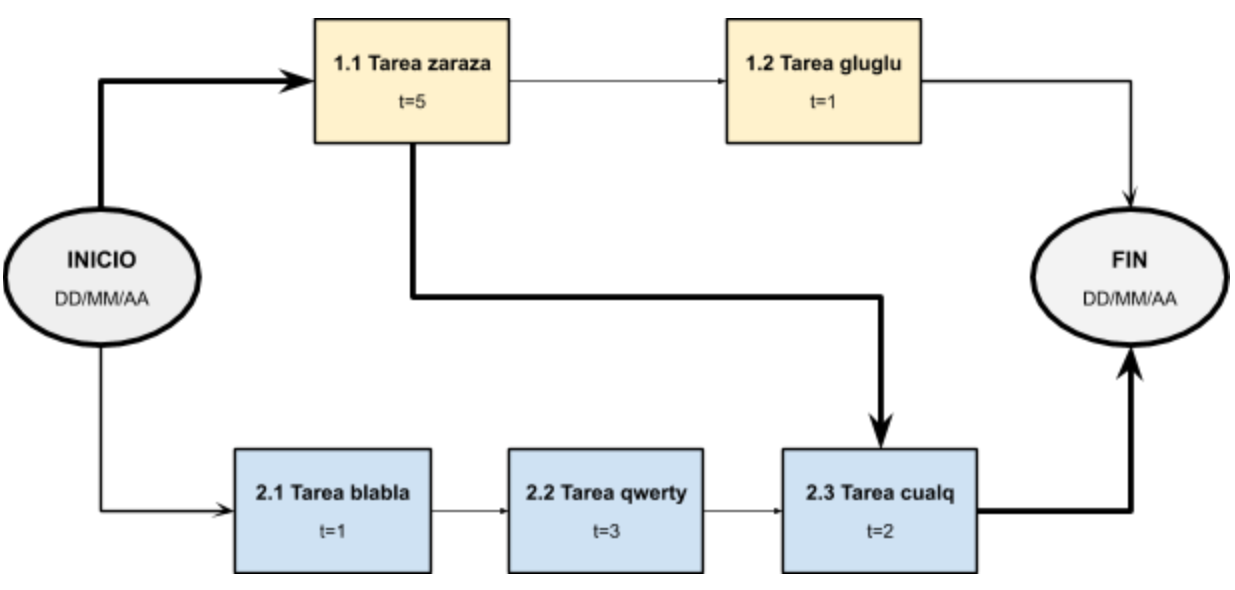
\includegraphics[width=.8\textwidth]{./Figuras/AoN.png}
\caption{Diagrama en \textit{Activity on Node}}
\label{fig:AoN}
\end{figure}

Indicar claramente en qué unidades están expresados los tiempos.
De ser necesario indicar los caminos semicríticos y analizar sus tiempos mediante un cuadro.
Es recomendable usar colores y un cuadro indicativo describiendo qué representa cada color, como se muestra en el siguiente ejemplo:



\section{8. Diagrama de Gantt}
\label{sec:gantt}

\begin{consigna}{red}
Utilizar el software Gantter for Google Drive o alguno similar para dibujar el diagrama de Gantt.

Existen muchos programas y recursos \textit{online} para hacer diagramas de gantt, entre las cuales destacamos:

\begin{itemize}
\item Planner
\item GanttProject
\item Trello + \textit{plugins}. En el siguiente link hay un tutorial oficial: \\ \url{https://blog.trello.com/es/diagrama-de-gantt-de-un-proyecto}
\item Creately, herramienta online colaborativa. \\\url{https://creately.com/diagram/example/ieb3p3ml/LaTeX}
\item Se puede hacer en latex con el paquete \textit{pgfgantt}\\ \url{http://ctan.dcc.uchile.cl/graphics/pgf/contrib/pgfgantt/pgfgantt.pdf}
\end{itemize}

Pegar acá una captura de pantalla del diagrama de Gantt, cuidando que la letra sea suficientemente grande como para ser legible. 
Si el diagrama queda demasiado ancho, se puede pegar primero la ``tabla'' del Gantt y luego pegar la parte del diagrama de barras del diagrama de Gantt.

Configurar el software para que en la parte de la tabla muestre los códigos del EDT (WBS).\\
Configurar el software para que al lado de cada barra muestre el nombre de cada tarea.\\
Revisar que la fecha de finalización coincida con lo indicado en el Acta Constitutiva.

En la figura \ref{fig:gantt}, se muestra un ejemplo de diagrama de gantt realizado con el paquete de \textit{pgfgantt}. En la plantilla pueden ver el código que lo genera y usarlo de base para construir el propio.

\begin{figure}[htbp]
\begin{center}
\begin{ganttchart}{1}{12}
  \gantttitle{2020}{12} \\
  \gantttitlelist{1,...,12}{1} \\
  \ganttgroup{Group 1}{1}{7} \\
  \ganttbar{Task 1}{1}{2} \\
  \ganttlinkedbar{Task 2}{3}{7} \ganttnewline
  \ganttmilestone{Milestone o hito}{7} \ganttnewline
  \ganttbar{Final Task}{8}{12}
  \ganttlink{elem2}{elem3}
  \ganttlink{elem3}{elem4}
\end{ganttchart}
\end{center}
\caption{Diagrama de gantt de ejemplo}
\label{fig:gantt}
\end{figure}

\end{consigna}

\section{9. Matriz de uso de recursos de materiales}
\label{sec:recursos}


\begin{table}
\label{tab:recursos}
\centering
\begin{tabularx}{\linewidth}{@{}|c|X|X|X|X|c|@{}}
\hline
\cellcolor[HTML]{C0C0C0} & \cellcolor[HTML]{C0C0C0} & \multicolumn{4}{c|}{\cellcolor[HTML]{C0C0C0}Recursos requeridos (horas)} \\ \cline{3-6} 
\multirow{-2}{*}{\cellcolor[HTML]{C0C0C0}\begin{tabular}[c]{@{}c@{}}Código\\ WBS\end{tabular}} & \multirow{-2}{*}{\cellcolor[HTML]{C0C0C0}\begin{tabular}[c]{@{}c@{}}Nombre \\ tarea\end{tabular}} & Material 1 & Material 2 & Material 3 & Material 4 \\ \hline
 &  &  &  &  &  \\ \hline
 &  &  &  &  &  \\ \hline
 &  &  &  &  &  \\ \hline
 &  &  &  &  &  \\ \hline
 &  &  &  &  &  \\ \hline
 &  &  &  &  &  \\ \hline
 &  &  &  &  &  \\ \hline
 &  &  &  &  &  \\ \hline 
 &  &  &  &  &  \\ \hline
 &  &  &  &  &  \\ \hline
 &  &  &  &  &  \\ \hline
 &  &  &  &  &  \\ \hline
 &  &  &  &  &  \\ \hline
 &  &  &  &  &  \\ \hline
 &  &  &  &  &  \\ \hline
 &  &  &  &  &  \\ \hline
 &  &  &  &  &  \\ \hline
 &  &  &  &  &  \\ \hline
 &  &  &  &  &  \\ \hline
 &  &  &  &  &  \\ \hline
 &  &  &  &  &  \\ \hline
 &  &  &  &  &  \\ \hline
 &  &  &  &  &  \\ \hline
 &  &  &  &  &  \\ \hline 
 &  &  &  &  &  \\ \hline
 &  &  &  &  &  \\ \hline
 &  &  &  &  &  \\ \hline
 &  &  &  &  &  \\ \hline

\end{tabularx}%
\end{table}


\section{10. Presupuesto detallado del proyecto}
\label{sec:presupuesto}

\begin{consigna}{red}
Si el proyecto es complejo entonces separarlo en partes:
\begin{itemize}
\item Un total global, indicando el subtotal acumulado por cada una de las áreas.
\item El desglose detallado del subtotal de cada una de las áreas.
\end{itemize}

IMPORTANTE: No olvidarse de considerar los COSTOS INDIRECTOS.

\end{consigna}

\begin{table}[htpb]
\centering
\begin{tabularx}{\linewidth}{@{}|X|c|r|r|@{}}
\hline
\rowcolor[HTML]{C0C0C0} 
\multicolumn{4}{|c|}{\cellcolor[HTML]{C0C0C0}COSTOS DIRECTOS} \\ \hline
\rowcolor[HTML]{C0C0C0} 
Descripción &
  \multicolumn{1}{c|}{\cellcolor[HTML]{C0C0C0}Cantidad} &
  \multicolumn{1}{c|}{\cellcolor[HTML]{C0C0C0}Valor unitario} &
  \multicolumn{1}{c|}{\cellcolor[HTML]{C0C0C0}Valor total} \\ \hline
 &
  \multicolumn{1}{c|}{} &
  \multicolumn{1}{c|}{} &
  \multicolumn{1}{c|}{} \\ \hline
 &
  \multicolumn{1}{c|}{} &
  \multicolumn{1}{c|}{} &
  \multicolumn{1}{c|}{} \\ \hline
\multicolumn{1}{|l|}{} &
   &
   &
   \\ \hline
\multicolumn{1}{|l|}{} &
   &
   &
   \\ \hline
\multicolumn{3}{|c|}{SUBTOTAL} &
  \multicolumn{1}{c|}{} \\ \hline
\rowcolor[HTML]{C0C0C0} 
\multicolumn{4}{|c|}{\cellcolor[HTML]{C0C0C0}COSTOS INDIRECTOS} \\ \hline
\rowcolor[HTML]{C0C0C0} 
Descripción &
  \multicolumn{1}{c|}{\cellcolor[HTML]{C0C0C0}Cantidad} &
  \multicolumn{1}{c|}{\cellcolor[HTML]{C0C0C0}Valor unitario} &
  \multicolumn{1}{c|}{\cellcolor[HTML]{C0C0C0}Valor total} \\ \hline
\multicolumn{1}{|l|}{} &
   &
   &
   \\ \hline
\multicolumn{1}{|l|}{} &
   &
   &
   \\ \hline
\multicolumn{1}{|l|}{} &
   &
   &
   \\ \hline
\multicolumn{3}{|c|}{SUBTOTAL} &
  \multicolumn{1}{c|}{} \\ \hline
\rowcolor[HTML]{C0C0C0}
\multicolumn{3}{|c|}{TOTAL} &
   \\ \hline
\end{tabularx}%
\end{table}


\section{11. Matriz de asignación de responsabilidades}
\label{sec:responsabilidades}
\begin{consigna}{red}
Establecer la matriz de asignación de responsabilidades y el manejo de la autoridad completando la siguiente tabla:

\begin{table}[htpb]
\centering
\resizebox{\textwidth}{!}{%
\begin{tabular}{|c|c|c|c|c|c|}
\hline
\rowcolor[HTML]{C0C0C0} 
\cellcolor[HTML]{C0C0C0} &
  \cellcolor[HTML]{C0C0C0} &
  \multicolumn{4}{c|}{\cellcolor[HTML]{C0C0C0}Listar todos los nombres y roles del proyecto} \\ \cline{3-6} 
\rowcolor[HTML]{C0C0C0} 
\cellcolor[HTML]{C0C0C0} &
  \cellcolor[HTML]{C0C0C0} &
  Responsable &
  Orientador &
  Equipo &
  Cliente \\ \cline{3-6} 
\rowcolor[HTML]{C0C0C0} 
\multirow{-3}{*}{\cellcolor[HTML]{C0C0C0}\begin{tabular}[c]{@{}c@{}}Código\\ WBS\end{tabular}} &
  \multirow{-3}{*}{\cellcolor[HTML]{C0C0C0}Nombre de la tarea} &
  \authorname &
  \supname &
  Nombre de alguien &
  \clientename \\ \hline
 &  &  &  &  &  \\ \hline
 &  &  &  &  &  \\ \hline
 &  &  &  &  &  \\ \hline
\end{tabular}%
}
\end{table}

{\footnotesize
Referencias:
\begin{itemize}
	\item P = Responsabilidad Primaria
	\item S = Responsabilidad Secundaria
	\item A = Aprobación
	\item I = Informado
	\item C = Consultado
\end{itemize}
} %footnotesize

Una de las columnas debe ser para el Director, ya que se supone que participará en el proyecto.
A su vez se debe cuidar que no queden muchas tareas seguidas sin ``A'' o ``I''.

Importante: es redundante poner ``I/A'' o ``I/C'', porque para aprobarlo o responder consultas primero la persona debe ser informada.

\end{consigna}

\section{12. Gestión de riesgos}
\label{sec:riesgos}

\begin{consigna}{red}
a) Identificación de los riesgos (al menos cinco) y estimación de sus consecuencias:
 
Riesgo 1: detallar el riesgo (riesgo es algo que si ocurre altera los planes previstos)
\begin{itemize}
\item Severidad (S): mientras más severo, más alto es el número (usar números del 1 al 10).\\
Justificar el motivo por el cual se asigna determinado número de severidad (S).
\item Probabilidad de ocurrencia (O): mientras más probable, más alto es el número (usar del 1 al 10).\\
Justificar el motivo por el cual se asigna determinado número de (O). 
\end{itemize}   

Riesgo 2:
\begin{itemize}
\item Severidad (S): 
\item Ocurrencia (O):
\end{itemize}

Riesgo 3:
\begin{itemize}
\item Severidad (S): 
\item Ocurrencia (O):
\end{itemize}


b) Tabla de gestión de riesgos:      (El RPN se calcula como RPN=SxO)

\begin{table}[htpb]
\centering
\begin{tabularx}{\linewidth}{@{}|X|c|c|c|c|c|c|@{}}
\hline
\rowcolor[HTML]{C0C0C0} 
Riesgo & S & O & RPN & S* & O* & RPN* \\ \hline
       &   &   &     &    &    &      \\ \hline
       &   &   &     &    &    &      \\ \hline
       &   &   &     &    &    &      \\ \hline
       &   &   &     &    &    &      \\ \hline
       &   &   &     &    &    &      \\ \hline
\end{tabularx}%
\end{table}

Criterio adoptado: 
Se tomarán medidas de mitigación en los riesgos cuyos números de RPN sean mayores a...

Nota: los valores marcados con (*) en la tabla corresponden luego de haber aplicado la mitigación.

c) Plan de mitigación de los riesgos que originalmente excedían el RPN máximo establecido:
 
Riesgo 1: plan de mitigación (si por el RPN fuera necesario elaborar un plan de mitigación).
  Nueva asignación de S y O, con su respectiva justificación:
  - Severidad (S): mientras más severo, más alto es el número (usar números del 1 al 10).
          Justificar el motivo por el cual se asigna determinado número de severidad (S).
  - Probabilidad de ocurrencia (O): mientras más probable, más alto es el número (usar del 1 al 10).
          Justificar el motivo por el cual se asigna determinado número de (O).

Riesgo 2: plan de mitigación (si por el RPN fuera necesario elaborar un plan de mitigación).
 
Riesgo 3: plan de mitigación (si por el RPN fuera necesario elaborar un plan de mitigación).

\end{consigna}


\section{13. Gestión de la calidad}
\label{sec:calidad}

\begin{consigna}{red}
Para cada uno de los requerimientos del proyecto indique:
\begin{itemize} 
\item Req \#1: copiar acá el requerimiento.

Verificación y validación:

\begin{itemize}
\item Verificación para confirmar si se cumplió con lo requerido antes de mostrar el sistema al cliente. Detallar 
\item Validación con el cliente para confirmar que está de acuerdo en que se cumplió con lo requerido. Detallar  
\end{itemize}

\end{itemize}

Tener en cuenta que en este contexto se pueden mencionar simulaciones, cálculos, revisión de hojas de datos, consulta con expertos, mediciones, etc.

\end{consigna}

\section{14. Comunicación del proyecto}
\label{sec:comunicaciones}

El plan de comunicación del proyecto es el siguiente:

\begin{table}[htpb]
\centering
\begin{tabularx}{\linewidth}{@{}|X|C{2.4cm}|C{3cm}|C{1.8cm}|C{2cm}|C{2.1cm}|@{}}
\hline
\rowcolor[HTML]{C0C0C0} 
\multicolumn{6}{|c|}{\cellcolor[HTML]{C0C0C0}PLAN DE COMUNICACIÓN DEL PROYECTO}           \\ \hline
\rowcolor[HTML]{C0C0C0} 
¿Qué comunicar? & Audiencia & Propósito & Frecuencia & Método de comunicac. & Responsable \\ \hline
                &           &           &            &                      &             \\ \hline
                &           &           &            &                      &             \\ \hline
                &           &           &            &                      &             \\ \hline
                &           &           &            &                      &             \\ \hline
                &           &           &            &                      &             \\ \hline
\end{tabularx}
\end{table}

\section{15. Gestión de compras}
\label{sec:compras}

\begin{consigna}{red}
En caso de tener que comprar elementos o contratar servicios:
a) Explique con qué criterios elegiría a un proveedor.
b) Redacte el Statement of Work correspondiente.
\end{consigna}

\section{16. Seguimiento y control}
\label{sec:seguimiento}

\begin{consigna}{red}
Para cada tarea del proyecto establecer la frecuencia y los indicadores con los se seguirá su avance y quién será el responsable de hacer dicho seguimiento y a quién debe comunicarse la situación (en concordancia con el Plan de Comunicación del proyecto).

El indicador de avance tiene que ser algo medible, mejor incluso si se puede medir en \% de avance. Por ejemplo,se pueden indicar en esta columna cosas como ``cantidad de conexiones ruteadeas'' o ``cantidad de funciones implementadas'', pero no algo genérico y ambiguo como ``\%'', porque el lector no sabe porcentaje de qué cosa.

\end{consigna}

\begin{longtable}{|m{1cm}|m{3.5cm}|m{2.2cm}|m{2cm}|m{3cm}|m{1.5cm}|}
\hline
\rowcolor[HTML]{C0C0C0} 
\multicolumn{6}{|c|}{\cellcolor[HTML]{C0C0C0}SEGUIMIENTO DE AVANCE}                                                                       \\ \hline
\rowcolor[HTML]{C0C0C0} 
Tarea del WBS 			& Indicador de avance & Frecuencia de reporte & Resp. de seguimiento & Persona a ser informada & Método de comunic. \\ \hline
\endfirsthead

\hline
\rowcolor[HTML]{C0C0C0} 
\multicolumn{6}{c}{\cellcolor[HTML]{C0C0C0}SEGUIMIENTO DE AVANCE}                                                                       \\ \hline
\rowcolor[HTML]{C0C0C0} 
Tarea del WBS 			& Indicador de avance & Frecuencia de reporte & Resp. de seguimiento & Persona a ser informada & Método de comunic. \\ \hline
\endhead

\multicolumn{6}{c}{Continúa}
\endfoot

\endlastfoot

1.1	& Fecha de inicio  & Única vez al comienzo & \authorname & \clientename, \supname & email \\ \hline
2.1	& Avance de las subtareas  & Mensual mientras dure la tarea & \authorname & \clientename, \supname & email \\ \hline

\end{longtable}

\begin{table}[!htpb]
\centering
%\begin{tabularx}{\linewidth}{@{}|X|X|X|X|X|X|@{}}
\begin{tabularx}{\linewidth}{@{}|X|C{2.5cm}|C{3cm}|C{2cm}|C{2cm}|C{2.5cm}|@{}}
\hline
\rowcolor[HTML]{C0C0C0} 
\multicolumn{6}{|c|}{\cellcolor[HTML]{C0C0C0}SEGUIMIENTO DE AVANCE}                                                                       \\ \hline
\rowcolor[HTML]{C0C0C0} 
Tarea del WBS & Indicador de avance & Frecuencia de reporte & Resp. de seguimiento & Persona a ser informada & Método de comunic. \\ \hline
 &  &  &  &  &  \\ \hline
 &  &  &  &  &  \\ \hline
 &  &  &  &  &  \\ \hline
 &  &  &  &  &  \\ \hline
 &  &  &  &  &  \\ \hline
\end{tabularx}%
%}
\end{table}

\section{17. Procesos de cierre}    
\label{sec:cierre}

\begin{consigna}{red}
Establecer las pautas de trabajo para realizar una reunión final de evaluación del proyecto, tal que contemple las siguientes actividades:

\begin{itemize}
\item Pautas de trabajo que se seguirán para analizar si se respetó el Plan de Proyecto original:
 - Indicar quién se ocupará de hacer esto y cuál será el procedimiento a aplicar. 
\item Identificación de las técnicas y procedimientos útiles e inútiles que se utilizaron, y los problemas que surgieron y cómo se solucionaron:
 - Indicar quién se ocupará de hacer esto y cuál será el procedimiento para dejar registro.
\item Indicar quién organizará el acto de agradecimiento a todos los interesados, y en especial al equipo de trabajo y colaboradores:
  - Indicar esto y quién financiará los gastos correspondientes.
\end{itemize}

\end{consigna}


\end{document}
